\section{Мощения}
\vspace{-0.7cm}
\centerline{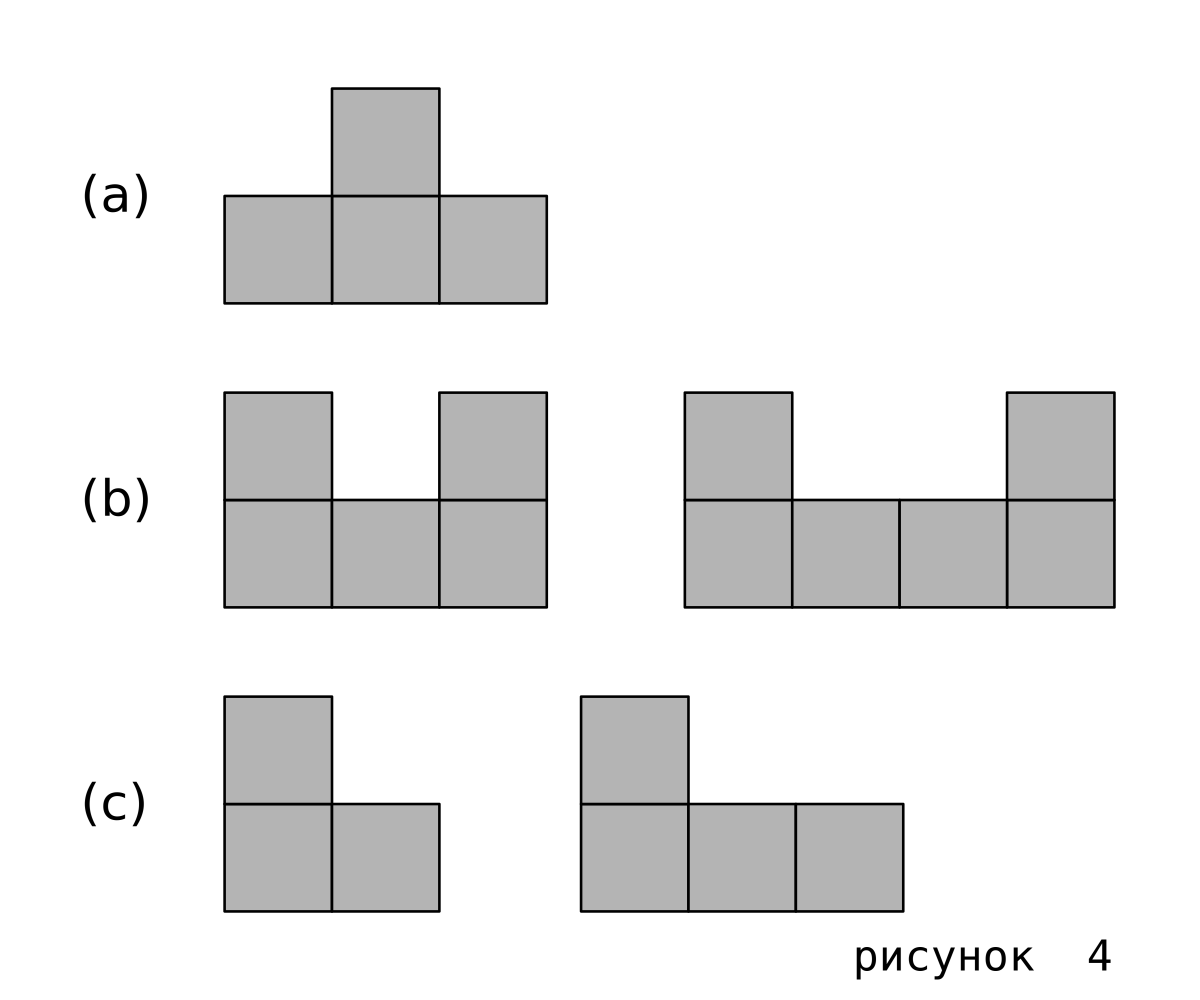
\includegraphics[width=5.5cm]{images/plane-park}}

\begin{enumerate}
\itA Укажите, как замостить плоскость фигурой с рисунка 4{\it (a)}.

\itB Укажите способ замощения плоскости каждой из двух фигур на рисунке 4{\it (b)}.

\itC Можно ли сложить квадрат какого-либо размера из деревянных плиток в форме фигур, изображённых на рисунке 4{\it (c)}? При этом необходимо пользоваться плитками обеих форм.
\end{enumerate}